% !TEX root = ../foresight.tex

\section{Planning for exploration}

Break into subsections:

Definitions.

Algorithm

Proofs


\begin{figure}
    \centering
    % 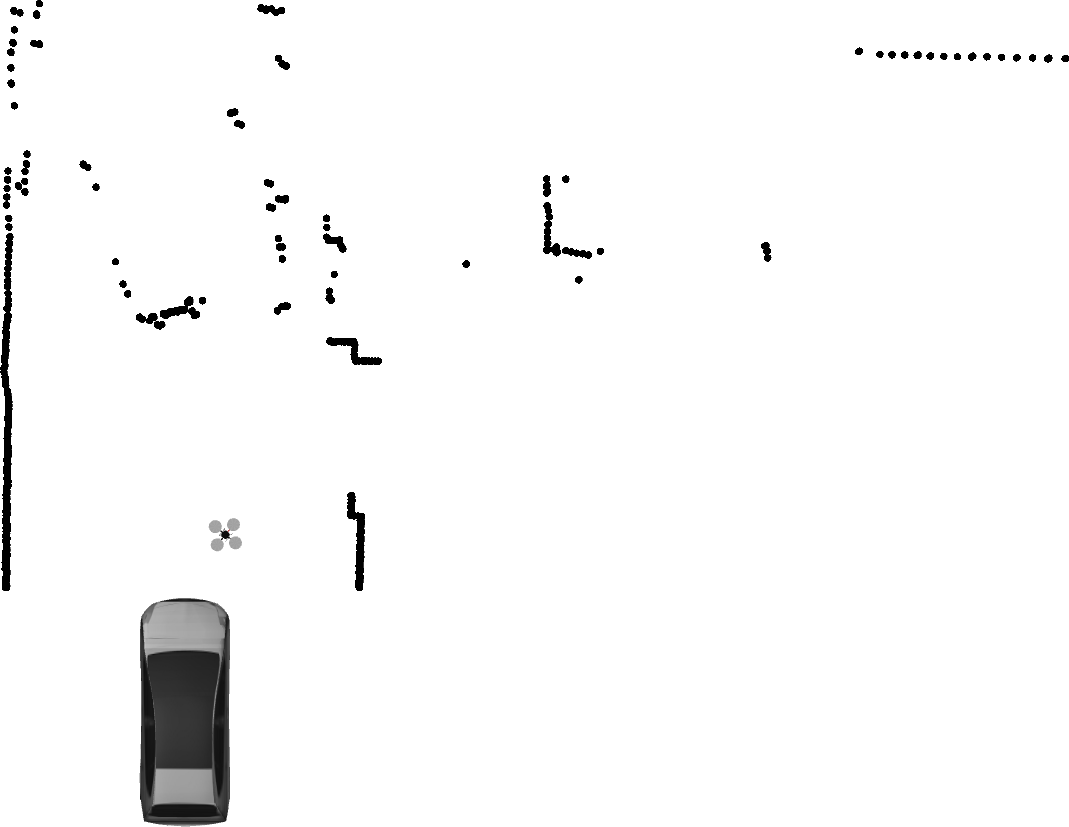
\includegraphics[width=0.49\linewidth]{01laser}
    % 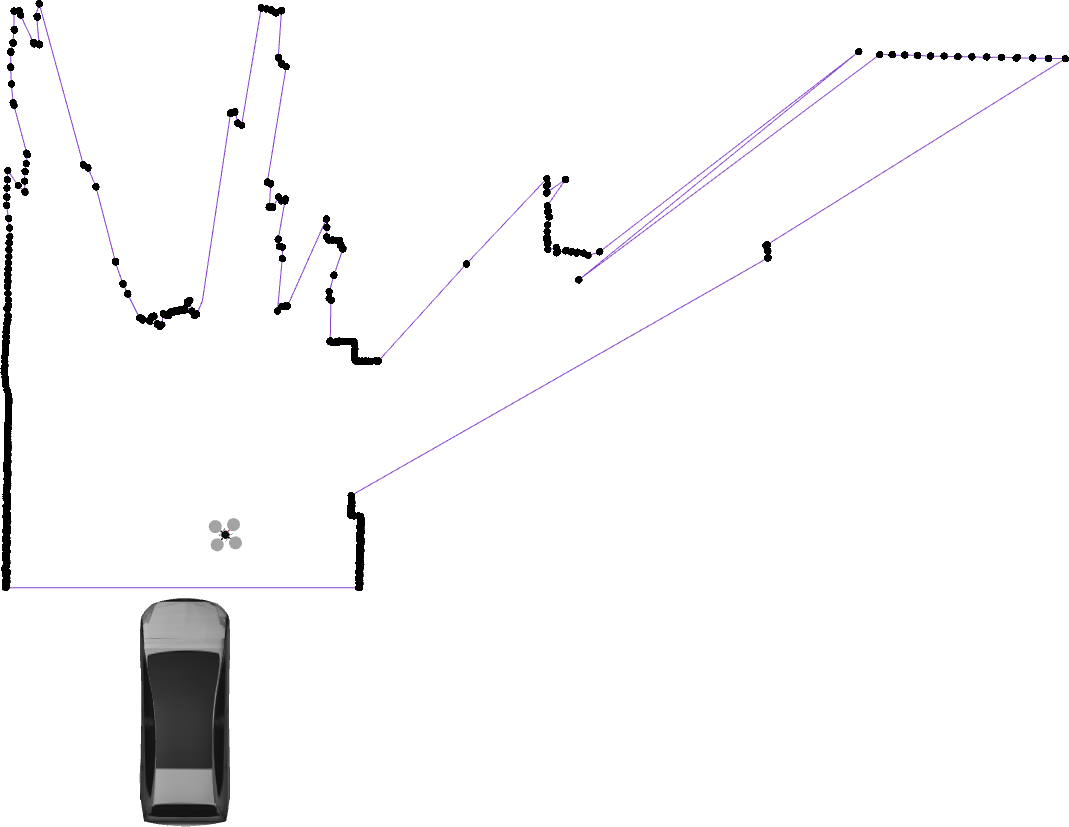
\includegraphics[width=0.49\linewidth]{02polygon} \\
    % 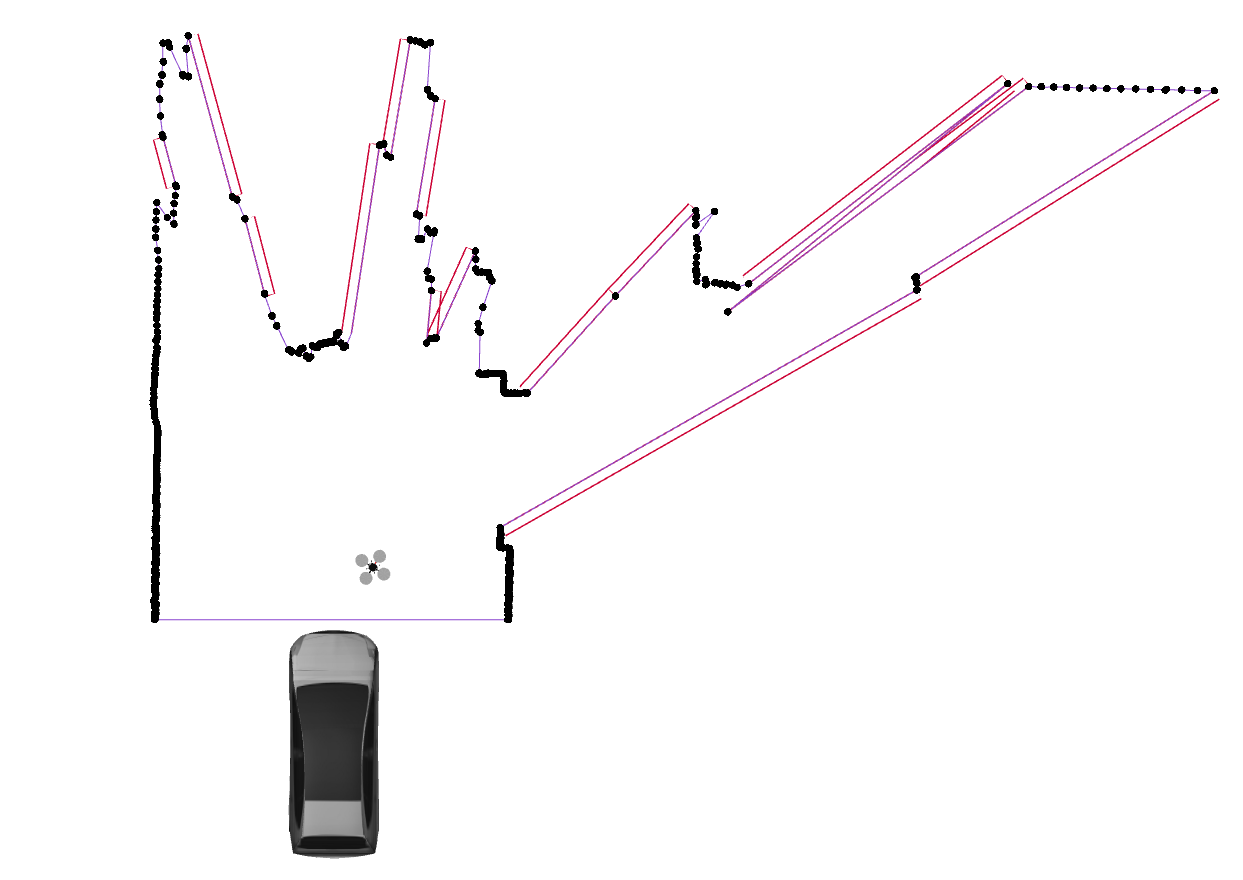
\includegraphics[width=0.49\linewidth]{03blindspots}
    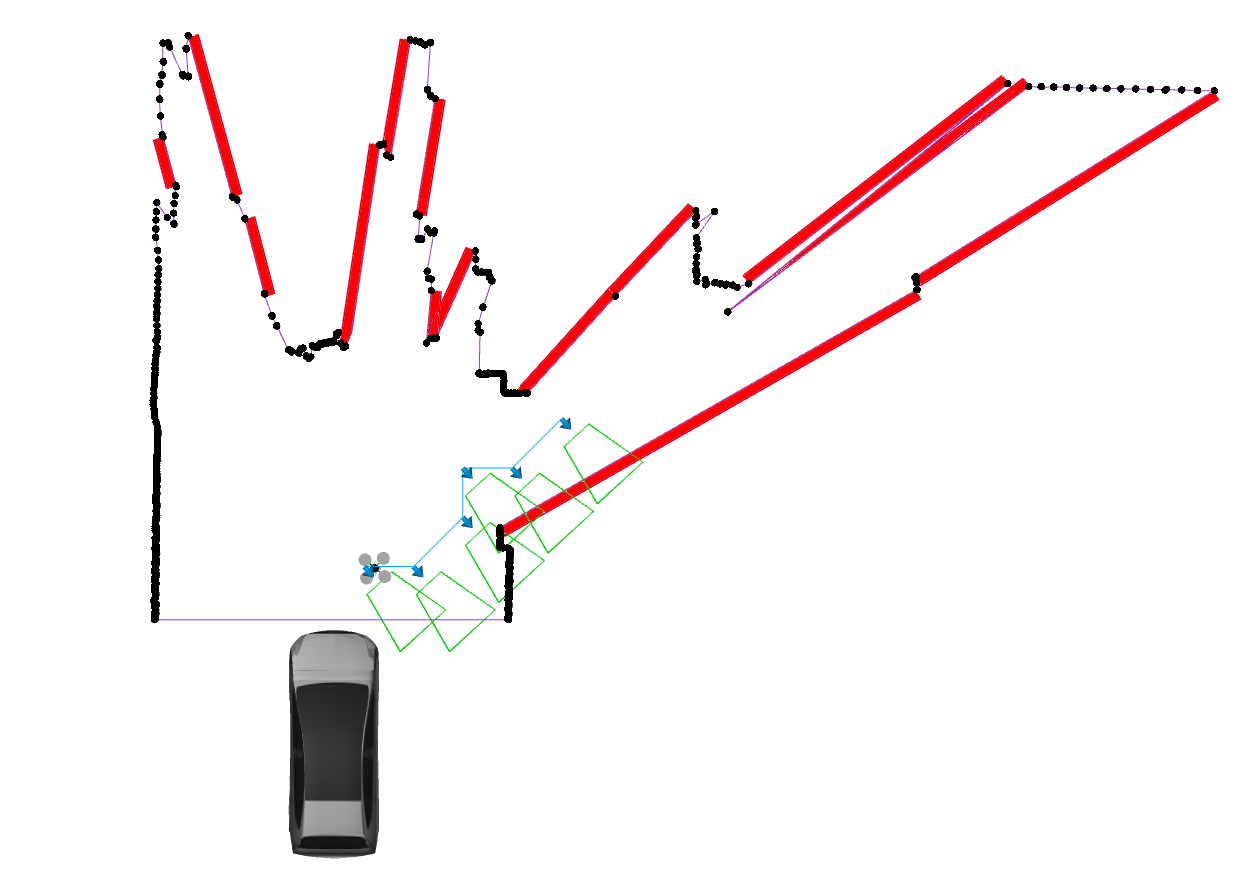
\includegraphics[width=1\linewidth]{04planner}
\end{figure}

\begin{definition}

    A laser scan is a sequence of points, $L \subset \R^2$, such that
    if a polygon, $P$, is constructed with these points, there exists a point,
    $c \in \R^2$, such that $\forall x \in L$, the line segment from
    $c$ to $x$ is entirely contained in $P$.

\end{definition}

\begin{definition}

    A break in the laser scan is a line segment $(L_i, L_{i + 1})$ such that
    $||L_i - L_{i + 1}||_2 > \delta$ where $\delta$ is the break threshold. The
    set of all these breaks will be referred to as $\tilde L$.

\end{definition}

\begin{definition}

    A blind spot, $B(L_i, L_{i + 1})$, is the set of points contained between
    the line segments, $(L_i, L_{i + 1})$ and $(L_i + \epsilon \cdot \hat n,
    L_{i + 1} + \epsilon \cdot \hat n)$ where $\hat n$ is the unit normal of
    the line segment $(L_i, L_{i + 1})$, $\epsilon$ is a parameter governing
    the size of the region, and $(L_i, L_{i + 1})$ is a break in the laser
    scan.

\end{definition}

\begin{definition}

    The blind region, $\mathcal{B}$, for a laser scan, $L$, is defined as
    $\mathcal{B} = \bigcup_{(i, j) \in \tilde L} B(i, j)$.

\end{definition}

\begin{definition}

    The sensor projection for our robot, $\psi(x, \theta)$ is defined as the
    set of points that the robot is able to observe from configuration $x$ with
    yaw, $\theta$. The optimal sensor projection for a given configuration and
    blind region is defined as $\psi^*(x, \B) = \psi(x, \theta^*(x, \B))$ with
    $\theta^*(x, \B) = \argmax{0 < \theta \leq 2\pi} \Area(\B \cap \psi(x,
    \theta))$

\end{definition}

\begin{definition}

    A path, $\rho \subset V \times [0, 2 \pi]$, is a sequence of tuples, $(x,
    \theta)$, consisting of state and yaw, such that $\forall
    i : (\rho_{i, x}, \rho_{i + 1, x}) \in E$, where $G = (V, E)$ is a finite
    sampled graph within the polygon constructed using the laser scan, $L$,
    that represents the connectivity of the free space.

\end{definition}

\begin{algorithm}[h!]
    \caption{}
    \algorithmicrequire{\begin{itemize}
            \item $x_0$: The initial position of the robot
            \item $\B$: The blind region
            \item $G = (V, E)$: The finite sampled graph within the laser scan
                polygon
            \item $\gamma$, $C$: The optimality and cumulative cost thresholds
                respectively for the algorithm's termination
        \end{itemize}}
    \algorithmicensure{\begin{itemize}
            \item $\rho \subset V \times [0, 2\pi]$: A sequence of tuples
                representing the path 
        \end{itemize}}
    \label{algo:find_path}
    \begin{algorithmic}[1]
        \setcounter{ALC@line}{0}
        \vspace*{1mm}

        \STATE $Q \leftarrow \{(x_0, \B \, \backslash \, \psi^*(x_0, \B), 0)\}$
        \WHILE{$|Q| > 0$}
            \STATE $(x, \rB, c) \leftarrow \argmin{q \in Q} \Area(q_{\rB})$
            \IF{$\Area(\B \, \backslash \, \rB) > \gamma \cdot \Area(\B)$}
                \STATE $\rho \leftarrow \{\}, \, \hat x \leftarrow x', \,
                    \hat \B \leftarrow \rB, \, \hat c \leftarrow c$
                \WHILE{$\Function{HasParent}(\hat x, \hat B, \hat c)$}
                    \STATE $\rho \leftarrow \{(\hat x,
                        \theta^*(\hat x, \hat \B))\} \cup \rho$
                    \STATE $(\hat x, \hat \B, \hat c) \leftarrow
                        \Function{Parent}(\hat x, \hat \B, \hat c)$
                \ENDWHILE
                \RETURN $\rho$
            \ENDIF
            \FORALL{$x' \where (x, x') \in E$}
                \STATE $c' \leftarrow c + \Function{CostToGo}(x, x')$
                \IF{$c' < C$}
                    \STATE $Q \leftarrow Q \cup \{(x', \rB \, \backslash \,
                        \psi^*(x', \rB), c')\}$
                    \STATE $\Function{Parent}(x', \rB \, \backslash \,
                        \psi^*(x', \rB), c') \leftarrow (x, \rB, c)$
                \ENDIF
            \ENDFOR
            \STATE $Q \leftarrow Q \, \backslash \, (x, \rB, c)$
        \ENDWHILE
        \RETURN $\False$

    \end{algorithmic}
\end{algorithm}

\begin{lemma}

    \label{lemma:cost}

    If a path is returned from Algo.~\ref{algo:find_path}, it will have a total
    cost less than $C$.

\end{lemma}

\begin{proof}

    At each iteration, the cost to reach each neighbour of $x$ is computed.
    This is added to the total cost of current path. If the cost of the path
    from $x_0$ to $x'$ is larger than $C$, it is discarded from the search.
    Thus only path with cost less than $C$, can be returned from
    Algo.~\ref{algo:find_path}.

\end{proof}

\begin{lemma}
    
    \label{lemma:finite}

    Algo.~\ref{algo:find_path} will finish in a finite number of steps if
    $\forall (i, j) \in E: \Function{CostToGo}(i, j) \geq 1$ and $C < \infty$

\end{lemma}

\begin{proof}

    Since the cumulative cost being added to search is monotonically
    increasing, if a given path is not returned, its cost will eventually be
    greater than $C$ in a finite amount of time since, $C <
    \infty$ and all individual costs must be greater than 1. If no path is
    returned by the algorithm, it means that all paths in $G$ have not reached
    the optimality threshold with their costs being less than $C$. Since $G$ is
    a finite graph, there are a finite amount of paths and therefore, to
    determine if no path will be returned takes a finite number of steps. If a
    path is returned, Algo.~\ref{algo:find_path} is returning the first path
    that meets the optimality threshold which would occur before all paths in G
    are exhausted, thus returning in a finite number of steps.

\end{proof}

\begin{lemma}

    \label{lemma:res_area}

    At each iteration, the residual blind region, $\B_n = \B \, \backslash \,
    \bigcup\limits_{(x_i, \theta_i) \in \rho} \psi(x_i, \theta_i)$ where $\rho$
    is the path from $x_0$ to $x_n$.

\end{lemma}

\begin{proof}

    At the $n^{\text{th}}$, the blind region in the tuple being added to $Q$ is

    \begin{align*}
        \B_n = \B \, \backslash \, \psi^*(x_0, \B) \, \backslash \,
        \psi^*(x_1, \B_0)
        \backslash \ldots \backslash \psi^*(x_n, \B_{n - 1})
    \end{align*}

    where $\B_i$ is the residual blind region for the $i^{\text{th}}$ step in
    path. Now we can rearrange to produce

    \begin{align*}
        \B_n = \B \, \backslash \, \bigcup_{i = 0}^{n - 1} 
        \psi^*(x_i, \B_{i - 1}) \\
    \end{align*}

    Now since $\psi^*(x_i, \B_{i - 1}) =
    \psi(x_i, \theta^*(x_i, \B_{i - 1})) = \psi(x_i, \theta_i)$, because
    the optimal yaw is added to the path for a given residual blind region,

    \begin{align*}
        \B_n = \B \, \backslash \bigcup_{(x_i, \theta_i) \in \rho}
        \psi(x_i, \theta_i)
    \end{align*}

\end{proof}

\begin{theorem}

    If there exists a path, $\rho$, such that $\Function{Area}(\mathcal{B}
    \, \cap \, \bigcup_{(x, \theta) \in \rho} \psi(x, \theta)) >  \gamma \cdot
    \Function{Area}(\mathcal{B})$ and $\rho$ can be executed by the
    robot with a total cost less than $C$, Algo.~\ref{algo:find_path} will
    return such a path in a finite number of steps.
    
\end{theorem}

\begin{proof}

    Using Lemmas~\ref{lemma:cost} and~\ref{lemma:finite}, we know that any path
    returned from Algo.~\ref{algo:find_path} will have a total cost less than
    $C$ and it will be returned in a finite number steps.  We also know from
    Lemma~\ref{lemma:res_area}, that the blind region at the $n^{\text{th}}$
    iteration is $\B \, \backslash
        \bigcup_{(x_i,
            \theta_i) \in
    \rho} \psi(x_i, \theta_i)$. Now, note that,

    \begin{align*}
        \B \backslash \B_n &= \B \backslash (\B \, \backslash
        \bigcup_{(x_i, \theta_i) \in \rho} \psi(x_i, \theta_i)) \\
        &= \B \cap
        \bigcup_{(x_i, \theta_i) \in \rho} \psi(x_i, \theta_i)
    \end{align*}

    Now since, the algorithm only returns a path if $\Area(\B \backslash
    \B_n) > \gamma \cdot \Area(\B)$ and using the result above, the algorithm
    will only return a path such that $\Area(\B \cap
    \bigcup_{(x_i, \theta_i) \in \rho} \psi(x_i, \theta_i)) >
    \gamma \cdot \Area(\B)$

\end{proof}
